\section{系统变换域分析}

\subsection{三大变换关系}
\vspace{-3pt}
\begin{description}
\tightlist

\item[z-s映射] \(z = e^{st}\implies\begin{array}{c} r = e^{\sigma T} \\ \omega = \Omega T \end{array}\),T为采样周期

\vspace{-15pt}
\begin{figure}[H]
    \centering
    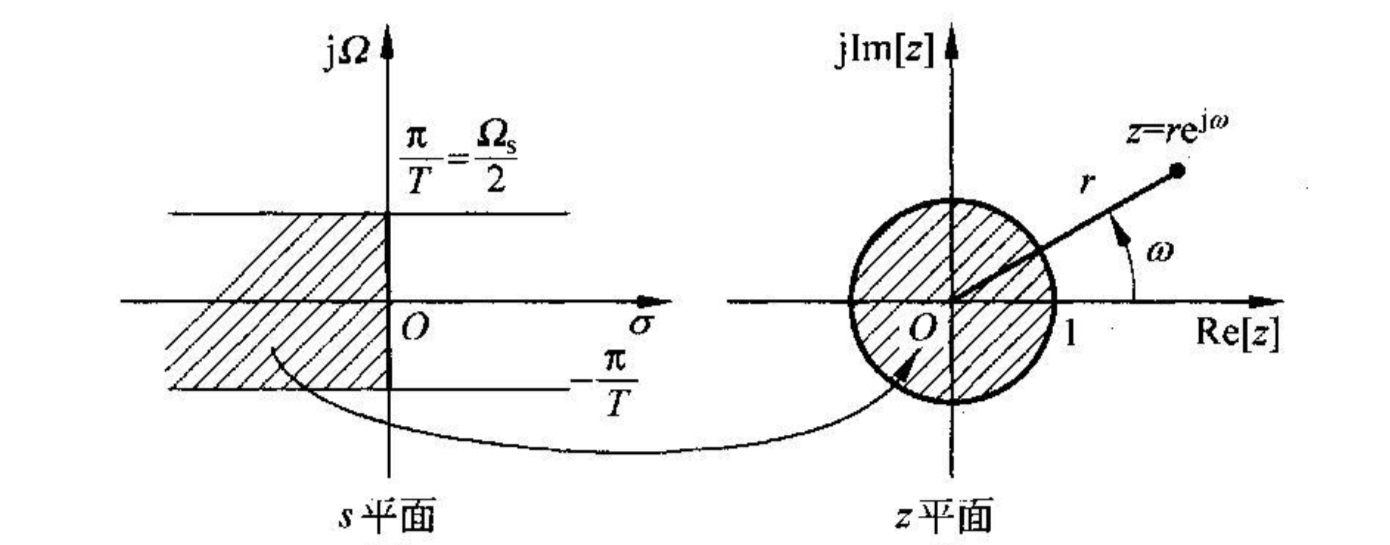
\includegraphics[width=\linewidth]{figure/IMG_48876557BC44-1.jpeg}
\end{figure}
\vspace{-15pt}

\item[DTFT] 单位圆上的Z变换
\(\mathcal F[x[n]] = X(e^{j\omega}) = \sum_{n=-\infty}^{+\infty} x[n] e^{-jn\omega}\)
\(x[n] = \frac{1}{2\pi} \int_{-\pi}^{\pi} X(e^{j\omega})e^{jn\omega}\D\omega\)

\{1,2,3,4,5,6,7\},N=5,\{7,9,3,4,5\}

\vspace{-10pt}
\begin{figure}[H]
    \centering
    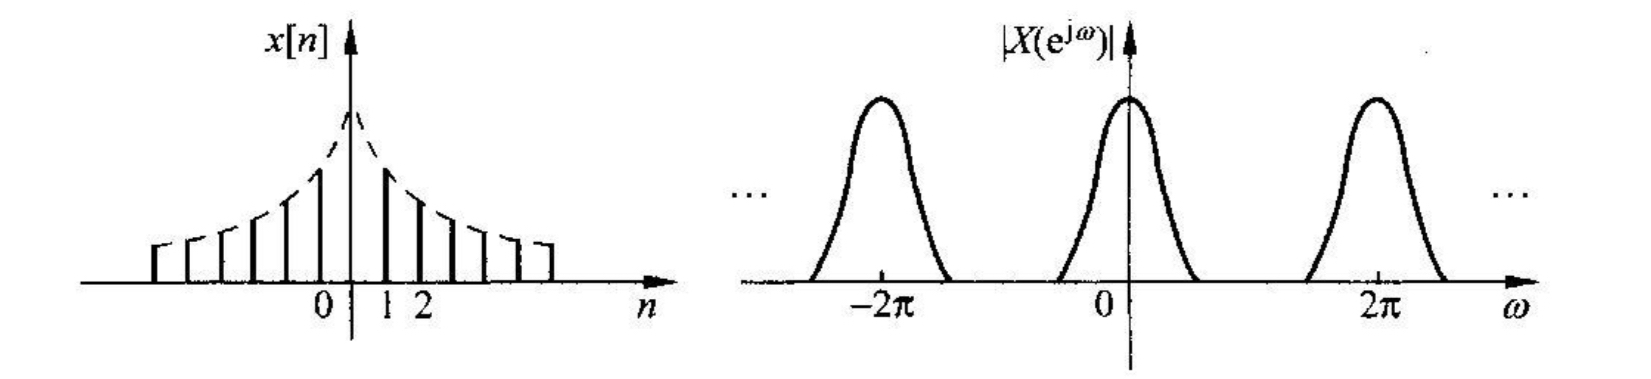
\includegraphics[width=\linewidth]{figure/IMG_CC52E79B1DEA-1.jpeg}
\end{figure}
\vspace{-20pt}

\end{description}


\subsection{系统函数}
\vspace{2pt}
\(H(z)=\frac{Y(z)}{X(z)}\quad h[n]\leftrightarrow H(z)\)

\vspace{-10pt}
\begin{table}[H]
    \tiny
    \setlength{\parskip}{0pt plus 0.5ex}
    \begin{tabular}{@{}ccc@{}}
    \toprule
    $h(t)$|$h[n]$ & $H(s)$ 极点 & $H(z)$ 极点 \\ \midrule
    衰减              & 左半平面        & 单位圆内        \\
    阶跃              & 原点          & 单位圆实轴交点    \\
    等幅震荡            & 虚轴,共轭       & 单位圆上,共轭     \\
    增长              & 右半平面        & 单位圆外        \\
    直流              & 实轴          & 正实轴         \\ \bottomrule
    \end{tabular}
\end{table}
\vspace{-10pt}

稳定系统:收敛域包含单位圆/虚轴\\
离散因果:\(z=\infty\)收敛(分子阶\(\leq\)分母阶)\\
连续因果:\(-\infty\)收敛,因果
因果稳定:极点全在单位圆内/左半平面

\vspace{-10pt}
\begin{table}[H]
    \tiny
    \setlength{\parskip}{0pt plus 0.5ex}
    \begin{tabular}{@{}cccc@{}}
    \toprule
    $h(t)$ & $H(s)$ 极点 & $H(z)$ 极点 & 稳定性 \\ \midrule
    衰减              & 左半平面        & 单位圆内        & 稳定  \\
    增长              & 右半平面        & 单位圆外        & 不稳定 \\
    增长              & 虚轴上多重极点     & 单位圆上多重    & 不稳定 \\
    等幅震荡            & 虚轴,共轭       & 单位圆上共轭     & 临界  \\
    阶跃              & 零点          & 单位圆实轴交点    & 临界  \\ \bottomrule
    \end{tabular}
\end{table}
\vspace{-10pt}


\vspace{-10pt}
\begin{figure}[H]
    \centering
    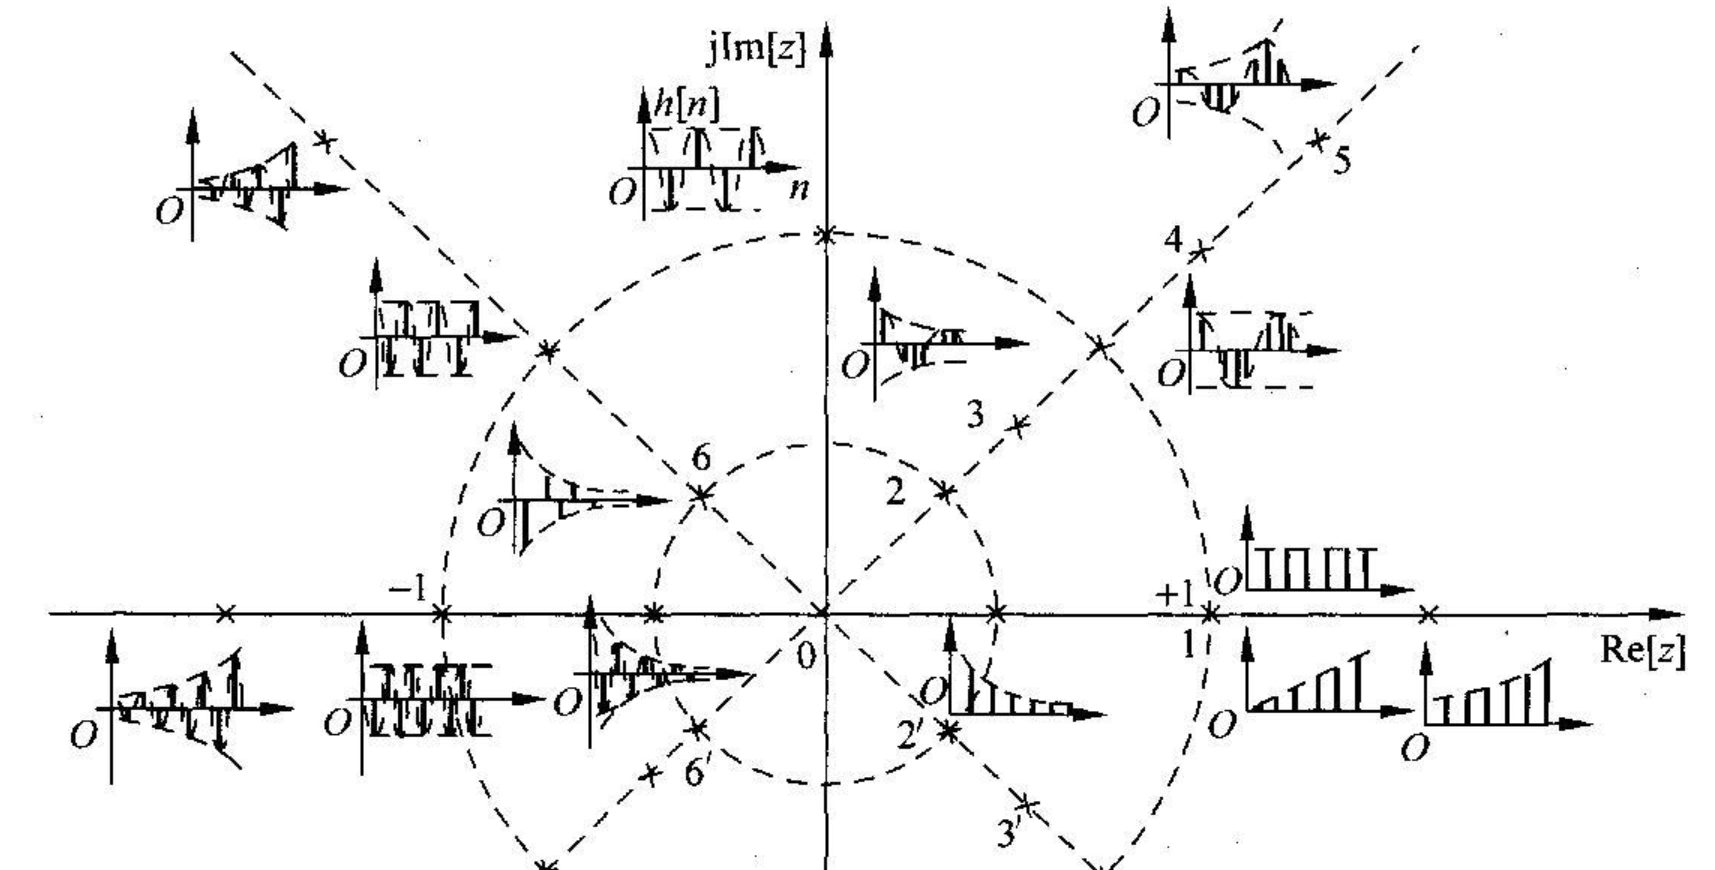
\includegraphics[width=\linewidth]{figure/Pasted image 20220612232835.png}
\end{figure}
\vspace{-10pt}
靠近原点振幅下降;向\(\pi\)运动频率上升。

\subsection{频率响应}

\(x[n] = e^{j\omega_0 n}\), \(y[n]=x[n]H(e^{j\omega_0})\),$H$ 的DTFT
\(H(e^{j\omega_0})=\|H(e^{j\omega_0})\|e^{j\varphi(\omega_0)}\),增益+相移

\vspace{-5pt}
\begin{description}
\tightlist
\item[几何确定] \(\left|\frac{H(e^{j\omega})}{K}\right| = \frac{\prod|\boldsymbol Z_j|}{\prod|\boldsymbol P_i|} = \frac{\text{零矢量模乘积}}{\text{极矢量模乘积}}\)
\(\varphi(\omega) = \sum \alpha_{z_j} - \sum \beta_{p_i} = \text{零矢幅角和} - \text{极矢幅角和}\)

\item[离散] 矢量终点 $\boldsymbol A$:$e^{j\omega}$,因此绕单位圆一周即可给出频响。(周期函数,$T=2\pi$)

\item[连续] \(H(j\Omega)\),矢量终点 $\boldsymbol A$ 从零点开始沿虚轴运动。$0\leq \Omega < \infty$

\end{description}

\subsection{相频特性}
单位圆内的零点,每转一圈,$\Delta\varphi(\omega) = 2\pi$\\
单位圆外的零点,每转一圈,$\Delta\varphi(\omega) = 0$

最小相位:唯一。\(M\)零点,\(2^M\)个同幅频特性。
\begin{description}
\tightlist

\item[全通]\(H_{ap}(z) = \frac{z^{-1}-z_0^*}{1-z_0z^{-1}}\)

连续:零极点分别位于虚轴左右,关于虚轴对称

\item[最小相位] 单位圆外/右半平面无零点 \\
每个周期内相频特性变化为零;
可以和全通系统级联表示非最小相位系统;
可逆;无负调现象。

\item[因果最小相位] 加上极点全在单位圆/左半平面

\vspace{-10pt}
\begin{figure}[H]
    \centering
    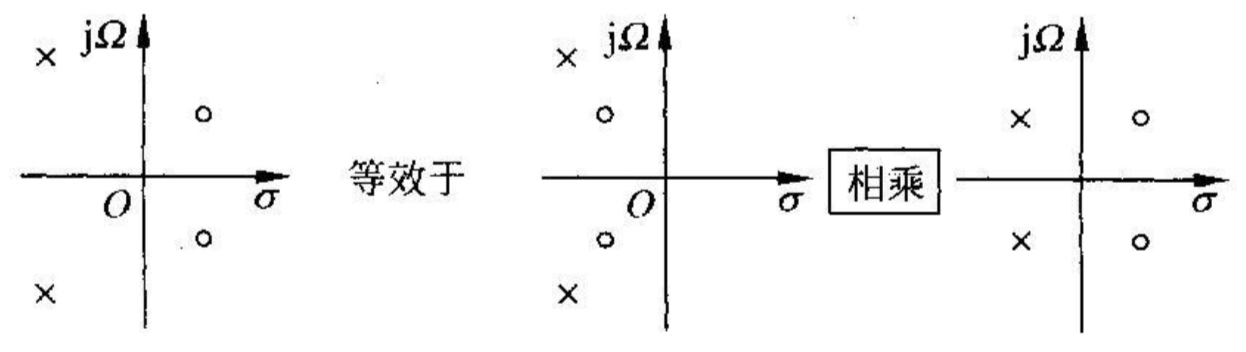
\includegraphics[width=\linewidth]{figure/IMG_EB82E9BC56FA-1.jpeg}
\end{figure}
\vspace{-10pt}
\end{description}
\vspace{-10pt}

% \vspace{-10pt}
% \begin{description}
% \tightlist
% \item[] 
% \end{description}